As mentioned in \refSec{sec_oz_dynamic_oz}, the mobility in Dynamic \oz{} is achieved
by attaching a distinguished variable transferableOperation for location. Location transferring
is mimicked by assigning a new location to that variable. To translate the variable \emph{transferableOperation} into the \picalc{} we cannot use \picalc{} channel as in \refSec{sec_tra_mapping_state_variables}, since the value of \emph{transferableOperation} will be a channel name and not a process representing a value like $Zero$. Thus, we map the variable transferableOperation to a channel named transferableOperation, where:

\begin{itemize}
\item transferableOperation = nil is mapped to Nullref(transferableOperation).

\item transferableOperation = talk is mapped to Ref(transferableOperation,talk).
\end{itemize}
as shown in \refFig{tra_ref} and \refLis{tra_ref_listing}.
\begin{figure}[H]%
\centering
\subcaptionbox{transferableOperation = nil.}{\fbox{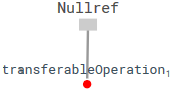
\includegraphics[keepaspectratio,width=0.45\textwidth]{./images/transformational_semantics_of_oz/transferableOperation_null.png}}}%
\hspace{\fill}
\hspace{1em}%
\subcaptionbox{transferableOperation = talk.}{\fbox{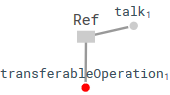
\includegraphics[keepaspectratio,width=0.45\textwidth]{./images/transformational_semantics_of_oz/transferableOperation.png}}}%
\caption{Mapping transferable operation's variable.}
\label{tra_ref}%
\end{figure}
\lstinputlisting[backgroundcolor=\color{white},caption={ Nullref and Ref processes in ABC code.},captionpos=b, label={tra_ref_listing}]{listings/ref_OZ.abc}
Thus, using the concept of transferable operation's variable we can now transform the classes \textit{IdleShop} and \textit{ActiveShop} as shown in \refFig{tra_idleShop_OZ}, \refLis{tra_idleShop_OZ_listing} and \refFig{tra_activeShop_OZ}, \refLis{tra_activeShop_OZ_listing}.
\begin{figure}[H]
\begin{subfigure}{.6\textwidth}
\centering
\begin{class}{IdleShop(id: \integer)}
\\
\begin{state}
self, vmId, message: \integer
\\transferableOperation: nil | talk
\end{state} 
\\
\begin{init}
\\self = id
\\transferableOperation = nil
\end{init} 
\\
\begin{op}{switch\_\_\_\_\ then\ ActiveShop}
\Delta (transferableOperation)
\\x?: nil | talk
\ST
x? = transferableOperation'
\end{op}
\end{class}
  \caption{IdleShop class in OZ}
\end{subfigure}%
\begin{subfigure}{.4\textwidth}
  \centering
\fbox{  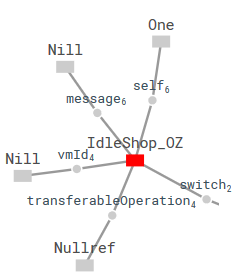
\includegraphics[width=.91\linewidth]{./images/transformational_semantics_of_oz/idleShop_OZ.png}}
  \caption{stargazer visualization}
\end{subfigure}
\caption{Transforming IdleShop into \picalc{} process IdleShop\_OZ\_PI}
\label{tra_idleShop_OZ}
\end{figure}

\lstinputlisting[backgroundcolor=\color{white},caption={The process IdleShop\_OZ\_PI in ABC code.},captionpos=b, label={tra_idleShop_OZ_listing}]{listings/idleShop_OZ.abc}
\begin{figure}[H]
\begin{subfigure}{.6\textwidth}
\centering
\begin{class}{ActiveShop(id: \integer)}
\\
\begin{state}
self, vmId, message: \integer
\\transferableOperation: nil | talk
\end{state} 
\\
\begin{init}
\\self = id
\\transferableOperation = talk
\end{init} 
\\
\begin{op}{switch\_\_\_\_\ then\ IdleShop}
x!: nil | talk
\ST
x! = transferableOperation
\\transferableOperation' = nil
\end{op}
\\
\begin{op}{talk}
\Delta (vmId, message)
\\y?, z?: \integer
\ST
y? = message'
\\z? = vmId'
\end{op}
\end{class}
  \caption{ActiveShop OZ class}
\end{subfigure}%
\begin{subfigure}{.4\textwidth}
  \centering
\fbox{  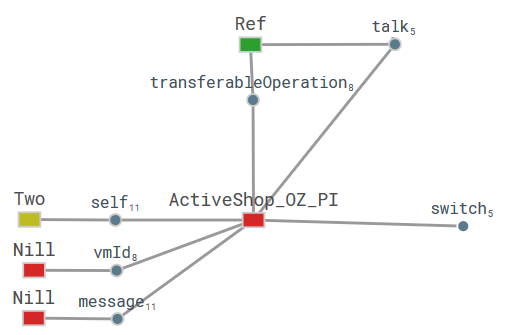
\includegraphics[width=.91\linewidth]{./images/transformational_semantics_of_oz/activeShop_OZ.png}}
  \caption{stargazer visualization}
\end{subfigure}
\caption{transforming ActiveShop into \picalc{} process ActiveShop\_OZ}
\label{tra_activeShop_OZ}
\end{figure}

\lstinputlisting[backgroundcolor=\color{white},caption={ ActiveShop OZ class as a process in ABC code.},captionpos=b, label={tra_activeShop_OZ_listing}]{listings/activeShop_OZ.abc}

Finally, \refFig{tra_system_before}, \refFig{tra_system_after} and \refLis{tra_system_lis} show the big picture of a system consisting of two shops, a vending machine and a customer. The full implementation can be found in the appendix.
\begin{figure}[H]%
\centering
\subcaptionbox{Before switching.}{\fbox{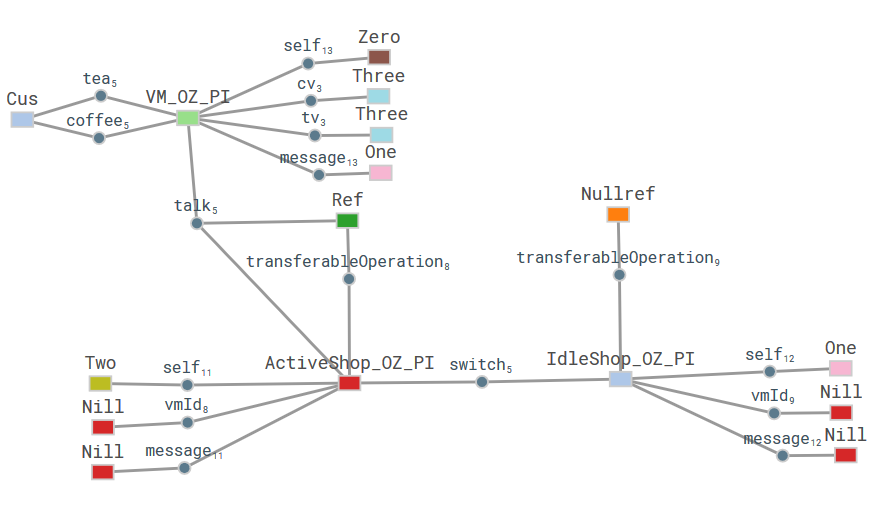
\includegraphics[keepaspectratio,width=0.45\textwidth]{./images/transformational_semantics_of_oz/all_switch_before.png}}}%
\hspace{1em}%
\subcaptionbox{After switching.}{\fbox{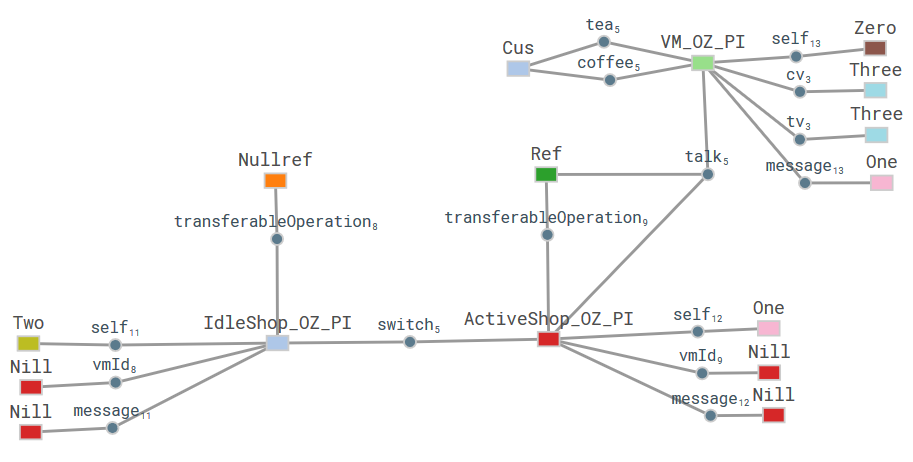
\includegraphics[keepaspectratio,width=0.45\textwidth]{./images/transformational_semantics_of_oz/all_after_switch.png}}}%
\caption{comparation as a process}
\label{tra_system}%
\end{figure}

\lstinputlisting[backgroundcolor=\color{white},caption={ system consisting of: two shops, vending machine and a customer.},captionpos=b, label={tra_system_lis}]{listings/system.abc}